\documentclass{article}
\usepackage[utf8]{inputenc}

% incluir imagens
\usepackage{graphicx}
\graphicspath{ {./images/} }

\title{Projeto Termômetro}
\author{Henrique Poleselo e Rodrigo Canário}
\date{March 2019}

\begin{document}

\maketitle

\section{Introdução}
O objetivo deste trabalho é integrar o conhecimento visto na disciplina Dispositivos Eletrônicos sobre diodos e reguladores de tensão juntamente com Eletrônica Digital para a implementação de circuitos em FPGA.
Usando um diodo semicondutor, seguindo a sua função característica do modelo real, conseguimos relacionar temperatura com os níveis de tensão aplicado ao mesmo. Partindo deste principio conseguimos construir um termomêtro digital.

\begin{center}
    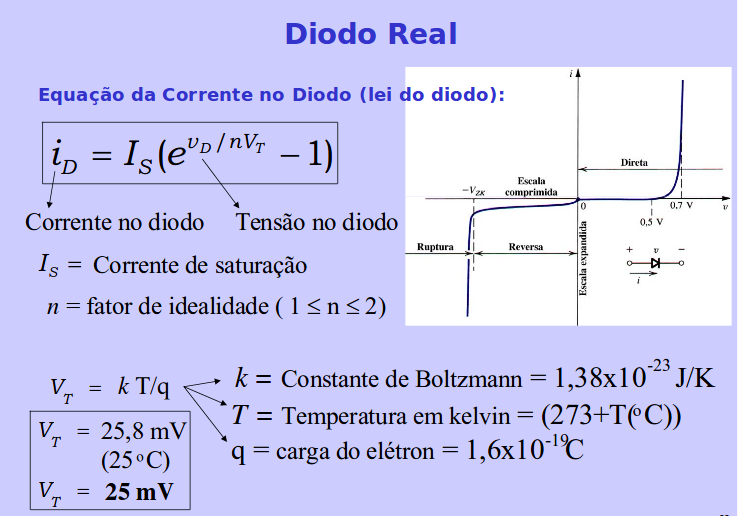
\includegraphics[scale=0.5]{images/img1.png}
    Imagem 1: Modelo do diodo real
\end{center}


\end{document}
